\subsection{Waveguides and Cavities}

\subsubsection{Electromagnetic Crosswalk}\label{Electromagnetic Crosswalk}

We have the following distribution of beams in the sketched intersection:

\begin{subequations}
	\begin{align}
		\vec{E_{H}} &= -E_{0} e^{i(kx - \omega t)} \hat{z}\\
		c \vec{B_{H}} &= E_{0} e^{i(kx - \omega t)} \hat{y}\\
		\vec{E_{V}} &= E_{0} e^{i(ky - \omega t)} \hat{z}\\
		c \vec{B_{V}} &= E_{0} e^{i(ky - \omega t)} \hat{x}
	\end{align}
\end{subequations}

\begin{figure}[h!]
	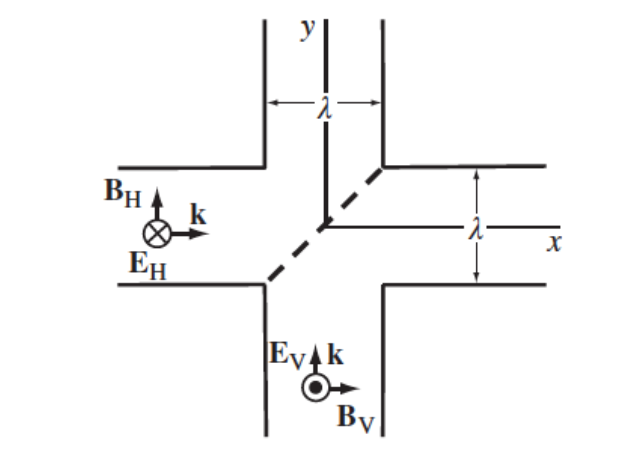
\includegraphics[width=6cm]{figures/crossbeams.png}
	\centering
	\caption{A sketch representation of the crossing beams and their components.}
\end{figure}

\textbf{a)}

The $\mathrm{H}$ and $\mathrm{V}$ beams are both propagating, monochromatic plane waves with electric field amplitude $E_{0}$. We know that the time-average density energy is given by:

\begin{equation}
	\langle u_{\mathrm{EM}} \rangle _{H, V}= \operatorname{Re}\left\{\frac{\epsilon_{0}}{4}\left(\mathbf{E} \cdot \mathbf{E}^{*}+c^{2} \mathbf{B} \cdot \mathbf{B}^{*}\right)\right\}=\frac{1}{2} \epsilon_{0} E_{0}^{2}.
\end{equation}

But at the very core of the intersection we are going to have a linear combination of $\mathbf{E}_{H}+\mathbf{E}_{V}$ and $\mathbf{B}_{H}+\mathbf{B}_{V}$, so this requires some computation to clean the following expression:
	
\begin{equation}
	\begin{split}
		\langle u_{\mathrm{EM}} \rangle_{\text{Total}}&= \operatorname{Re}\left\{\frac{\epsilon_{0}}{4}\left[\left(\mathbf{E}_{H}+\mathbf{E}_{V}\right) \cdot\left(\mathbf{E}_{H}^{*}+\mathbf{E}_{V}^{*}\right)+c^{2}\left(\mathbf{B}_{H}+\mathbf{B}_{H}\right) \cdot\left(\mathbf{B}_{H}^{*}+\mathbf{B}_{V}^{*}\right)\right]\right\}=\\
        &=\operatorname{Re}\left\{\frac{1}{4} \left( \epsilon_{0}\left(\mathbf{E}_{H}\mathbf{E}_{H}^{*} + \tfrac{1}{\epsilon_{0}\mu_{0}} \mathbf{B}_{H}\mathbf{B}_{H}^{*} \right)\right\}+\operatorname{Re}\left\{\frac{\epsilon_{0}}{4}\left(\mathbf{E}_{V}\mathbf{E}_{V}^{*} + \tfrac{1}{\epsilon_{0}\mu_{0}} \mathbf{B}_{V}\mathbf{B}_{V}^{*}\right) \right)\right\} +\\ 
		&\quad +\operatorname{Re}\left\{\frac{\epsilon_{0}}{4}\left(\mathbf{E}_{H}\mathbf{E}_{V}^{*} + \mathbf{E}_{V}\mathbf{E}_{H}^{*}+ \tfrac{1}{\epsilon_{0}\mu_{0}} \mathbf{B}_{H}\mathbf{B}_{V}^{*} +  \tfrac{1}{\epsilon_{0}\mu_{0}} \mathbf{B}_{V}\mathbf{B}_{H}^{*}\right)\right\}=\\
		&=\langle u_{\mathrm{EM}}\rangle_{H}+\langle u_{\mathrm{EM}}\rangle_{V}+\\
		&\quad+\operatorname{Re}\left\{\frac{\epsilon_{0}}{4}\left(\mathbf{E}_{H}\mathbf{E}_{V}^{*} + \mathbf{E}_{V}\mathbf{E}_{H}^{*}+ \tfrac{1}{\epsilon_{0}\mu_{0}} \mathbf{B}_{H}\mathbf{B}_{V}^{*} +  \tfrac{1}{\epsilon_{0}\mu_{0}} \mathbf{B}_{V}\mathbf{B}_{H}^{*}\right)\right\}. \\
	\end{split}
\end{equation}

Let us study some of the pieces of the last term in the previous line, so we can simplify even further. Observe that $\mathbf{B}_{H} \mathbf{B}_{V}^{*} = \mathbf{B}_{V} \mathbf{B}_{H}^{*} = 0$ because $\hat{y}\cdot \hat{x} = 0$. So the only possible contribution comes from:
	
\begin{equation}
	\mathbf{E}_{H} \mathbf{E}_{V}^{*} = - E_{0}^{2}\: e^{i(k x - ky)} \underbrace{\hat{z}\cdot\hat{z}}_{= 1}.
\end{equation}

And similarly for the other term with opposite sign in the exponent. So puting all together and recalling that $\left\langle u_{\mathrm{EM}}\right\rangle_{H, V}=\frac{1}{2} \epsilon_{0} E_{0}^{2}$, we have:
	
\begin{equation}
	\begin{split}
		\left\langle u_{\mathrm{EM}}\right\rangle_{Total}& =\tfrac{1}{2}\epsilon_{0} E_{0}^{2}+\tfrac{1}{2}\epsilon_{0} E_{0}^{2}-\tfrac{1}{2} \epsilon_{0} E_{0}^{2} \operatorname{Re}\underbrace{\left\{e^{i (k x - ky)} + e^{-i(kx- k y)}\right\}}_{=2 \cos(\arg)} =\\
		&=\tfrac{1}{2}\epsilon_{0} E_{0}^{2}\left[2- \cos (k\left[x-y\right])\right]
	\end{split}
\end{equation}

This quantity is minimum when $x=y$. On that plane (the diagonal of the crosswalk), the physical fields are:

\begin{equation}
	\mathbf{E}(x=y)=0 \hat{\mathbf{z}} \quad \text { and } \quad c \mathbf{B}(x=y)=E_{0} \cos (k x-\omega t)(\hat{\mathbf{x}}+\hat{\mathbf{y}})
\end{equation}

\textbf{b)}

Now we are asked to do exactly the same for the time-averaged Poynting vector for a plane wave propagating in the $\hat{\mathbf{k}}$ direction. This expression reads:

\begin{equation}
	\langle\mathbf{S}\rangle= \sqrt{\tfrac{\epsilon_{0}}{\mu_{0}}}|E_{0}|^{2}\hat{k}= c \left\langle u_{\mathrm{EM}}\right\rangle \hat{\mathbf{k}}.
\end{equation}

Therefore, the horizontal and vertical beams poynting expression follow from the previous part of the exercise as:

\begin{equation}
	\langle\mathbf{S}\rangle_{V}= c \epsilon_{0} E_{0}^{2} \hat{\mathbf{y}} \quad \text { and } \quad\langle\mathbf{S}\rangle_{H}= c \epsilon_{0} E_{0}^{2} \hat{\mathbf{x}}
\end{equation}

So the superposition reads:

\begin{equation}
	\begin{split}
		\langle\mathbf{S}\rangle &=\frac{1}{ \mu_{0}} \operatorname{Re}\left\{\left(\mathbf{E}_{H}+\mathbf{E}_{V}\right) \times\left(\mathbf{B}_{H}+\mathbf{B}_{V}\right)^{*}\right\}= \\
		&=\left\langle\mathbf{S}_{H}\right\rangle+\left\langle\mathbf{S}_{V}\right\rangle+\frac{1}{ \mu_{0}} \operatorname{Re}\left\{\mathbf{E}_{H} \times \mathbf{B}_{V}^{*}+\mathbf{E}_{V} \times \mathbf{B}_{H}^{*}\right\} =\\
		&= 2\: \epsilon_{0} \:c \: E_{0}^{2}(\hat{\mathbf{x}}+\hat{\mathbf{y}})-\frac{E_{0}^{2}  }{ \mu_{0}} \operatorname{Re}\underbrace{\left\{e^{i k(x-y)} \hat{\mathbf{y}}+e^{i k(y-x)} \hat{\mathbf{x}}\right\}}_{2\cos(\arg)} =\\
		&=2\:\epsilon_{0}\:c E_{0}^{2}[1- \cos k(x-y)](\hat{\mathbf{x}}+\hat{\mathbf{y}})
	\end{split}
\end{equation}

From this previous expression we can see that, again, something interesting will take place when $x=y$. Observe the following sketch. The Poynting vector grows outwards from the diagonal $x=y$.

\begin{figure}[h!]
	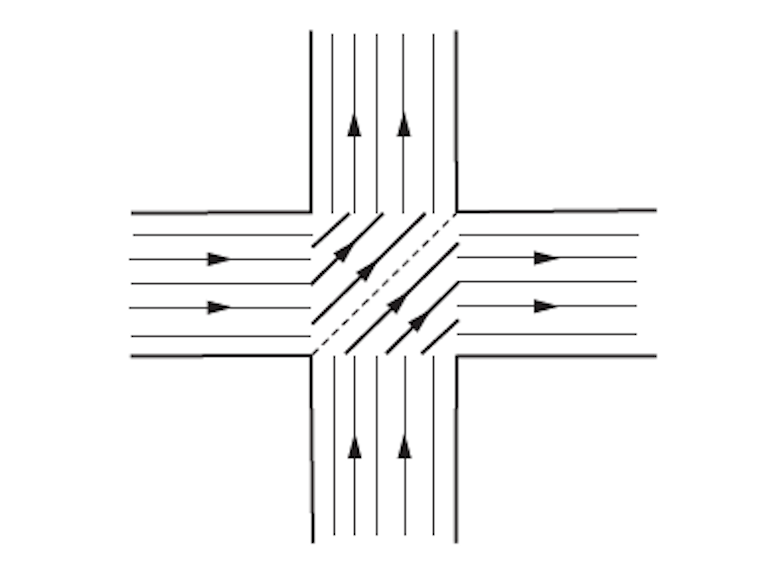
\includegraphics[width=6cm]{figures/electrocrosswalk.png}
	\centering
	\caption{The Poynting vector is nule in the $x=y$ diagonal.}
\end{figure}

\textbf{c)}

At the surface of a conductor, we must have $\mathbf{E}_{\|}=0$ and $\mathbf{B}_{\perp}=0$. For this problem, part (a) shows that $\mathbf{E}$ points along $\hat{\mathbf{z}}$ and goes to zero at $x=y .$ Part (a) showed also that $\mathrm{B}$ is parallel to the $x=y$ plane everywhere in the overlap region. Hence, the boundary conditions for a perfect conductor are met at $x=y$.

\subsubsection{Waveguide Discontinuity}\label{Waveguide Discontinuity}

The first question one has to ask is how the set-up looks like. It results to be something like the following:

\begin{figure}[h!]
	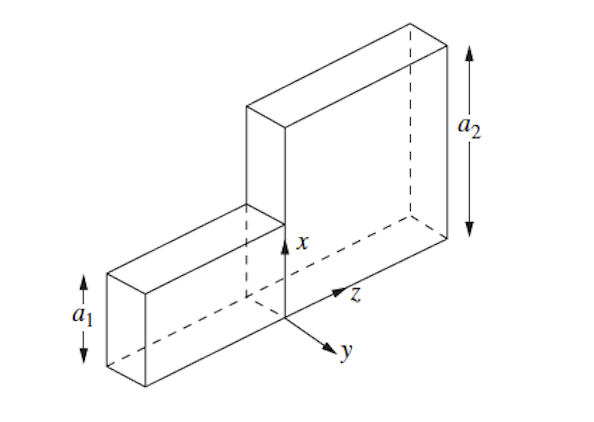
\includegraphics[width=7cm]{figures/waveguide_discontinuity.png}
	\centering
\end{figure}

Observe that $a_{2} > a_{1}$. The wave we want to study is moving from the region of $a_{1}$ to $a_{2}$. That difference of space will affect the modes of the wave, but how?

Recall that a $\mathrm{TE}$-mode means that $E_{\parallel} =0$ respect to the motion of the wave. This also implies that $\frac{\partial B_{z}}{\partial n}|_{s}=0$. For the subscript $1,0$ we refer to the specific mode of the solution we want to study. A general wave solution for a system like this goes as:

\begin{equation}
	\psi_{1} (x,y) = H_{m,n} \cos \left(\tfrac{m \pi x}{a_{1}}\right) \: \cos \left(\tfrac{n \pi y}{b}\right).
\end{equation}

For a $\mathrm{TE}_{m,0}$ mode in the first region, we have $\psi_{1} \propto \cos \left(m \pi x / a_{1}\right)$. As there is this change in height in the waveguide between the first and the second region, we do not know which new modes can or not appear. This can expressed as the following:

\begin{equation}
	\psi_{2} (x,y) = \sum_{m} \psi_{m,0} = \sum_{m} H_{m,0} \cos\left(\tfrac{m \pi x}{a_{2}}\right).
\end{equation}

The continuity of the tangential component of $\mathrm{E}$ shows that only $\mathrm{TE}_{m 0}$ modes will propagate in waveguide 2 because the absence of $y$ -dependence in guide 1 cannot generate $y$ -dependence in guide 2 . Our task, then, is to find the expansion coefficients $H_{m,0}$ so

\begin{equation}
	\psi_{2} = \sum_{m=1}^{\infty} H_{m,0} \cos \left(\frac{m \pi x}{a_{2}}\right)=\left\{\begin{array}{ll}
		H \cos \left(\pi x / a_{1}\right), & 0 \leq x \leq a_{1} \\
		0, & a_{1}<x \leq a_{2}
	\end{array}\right.
\end{equation}

where we refer to $H_{1,0}$ as $H$. This is a (quite dirty) job for the orthogonality properties of the cosine functions. Integrating we arrive to:

\begin{equation}
	\begin{split}
		H_{m,0} &=\frac{2 H}{a_{1}} \int_{0}^{a_{1}} d x \cos \left(\pi x / a_{1}\right) \cos \left(m \pi x / a_{2}\right)= \\
		&=\frac{2 H a_{2}}{\pi\left(a_{2}-m a_{1}\right)} \sin \left[\pi\left(1-m a_{1} / a_{2}\right)\right]-\frac{2 H a_{2}}{\pi\left(a_{2}+m a_{1}\right)} \sin \left[\pi\left(1+m a_{1} / a_{2}\right)\right] =\\
		&=\frac{2 H m a_{1} a_{2}}{\pi\left(a_{2}^{2}-m^{2} a_{1}^{2}\right)} \sin \left(m \pi \frac{a_{1}}{a_{2}}\right).
	\end{split}
\end{equation}

When $a_{1}=a_{2}, H_{m,0}=0$ for $m \neq 1$. When $m=1$, l'Hospital's rule gives the expected answer,

\begin{equation}
	H_{1,0}=\lim _{m \rightarrow 1} \frac{d}{d m} \frac{2 H}{\pi} \frac{\sin (m \pi)}{\left(1-m^{2}\right)}=\lim _{m \rightarrow 1} \frac{2 \pi H \cos (m \pi)}{-2 m \pi}=H.
\end{equation}

\subsubsection{Guess Who? (Wavefilter Edition)}\label{Guess Who? (Wavefilter Edition)}

Let first display how this two filters look like.

\begin{figure}[h!]
	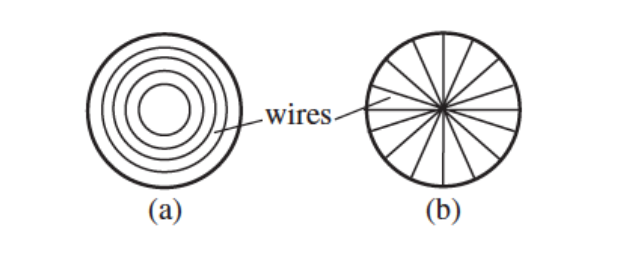
\includegraphics[width=8cm]{figures/2waveguides.png}
	\centering
\end{figure}

So we know that one has a $TM$- mode and the other one has a $TE$. Which is which?

Let's start from the basics. A general wave-guide will relate the $\mathbf{E}$ and $\mathbf{B}$ fields as:

\begin{equation}
	\vec{\nabla}\times\mathbf{E}_{\perp} = i \omega B_{z} \hat{z}.
\end{equation}

And the modes requirements imply:
\begin{equation}
	\begin{split}
		\mathrm{TM} \rightarrow B_{z} &= 0 \quad \text{and} \quad E_{z}|_{\mathrm{surface}} = 0,\\
		\mathrm{TE} \rightarrow E_{z} &= 0 \quad \text{and} \quad \tfrac{\partial B_{z}}{\partial n}|_{\mathrm{surface}} = 0.\\
	\end{split}
\end{equation}

In order to determine which mode correspond to which tube, let us choose the behavior of a $\mathrm{TM}$ mode, which implies then:

\begin{equation}
	\vec{\nabla} \times \mathbf{E}_{\perp} = 0 \quad \rightarrow \quad \vec{\nabla}\times \vec{\nabla}\cdot \phi = \vec{\nabla}\times (\partial_{x}\phi, \partial_{y} \phi, 0).
\end{equation}

This is giving us a hint. If we think in terms of small differences of the field $\phi$ in the $x,y$ directions, we see that there should not be any change. Hence, we can discard the possibility of this mode to be contained along those radial wires, which break the symmetry. This is not the case of the tube A, where $\Delta E|_{r=\mathrm{cnt}} = 0$. Then, $\mathrm{TM}$ corresponds to the tube A while $\mathrm{TE}$ mode corresponds to the tube B.

\subsubsection{An Electromagnetic Bat in a Resonant Cavity}\label{An Electromagnetic Bat in a Resonant Cavity}

In order to succesfully solve this problem we have to realise several things. The first one is that the combination of waves can be expressed as a linear combination of them as:

\begin{equation}
	\psi(x, y, t)=\sum_{m=0}^{n}(-1)^{m} \sin \left(\mathbf{k}_{m} \cdot \mathbf{r}-c k t\right),
\end{equation}\\
Where $n$ is the total number of waves. The second thing to realise is that $\mathrm{TM}$ modes in a cavity have the property that $\psi=0$ on the walls of the cavity. Instead of getting a reflection of the wave we emit\footnote{radar technology.}, we can sketch the inner structure of the cavity by using this anhilition property of the waves. We have to find the explicit expression of the L.C. of waves we have inside de cavity and solve a system of equations to determine the boundaries of this space. For that we need to compute $\mathbf{k}_{i}\cdot\mathbf{r}$.


\begin{figure}[h]
	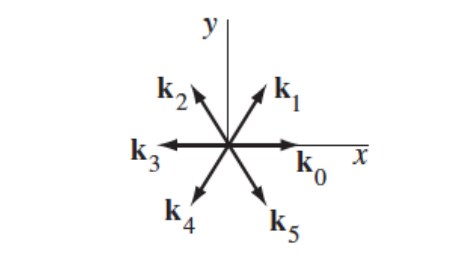
\includegraphics[width=8cm]{figures/6waves.png}
	\centering
	\caption{The vectorial distribution of the six waves.}
\end{figure}

\begin{equation}
	\begin{split}
		\mathbf{k}_{0} \cdot \mathbf{r}&=k x, \\
		\mathbf{k}_{1} \cdot \mathbf{r}&=\cos \left[\frac{\pi}{3}\right] k x+\sin \left[\frac{\pi}{3}\right] k y=\frac{1}{2} k x+\frac{\sqrt{3}}{2} k y,\\
		\mathbf{k}_{2} \cdot \mathbf{r}&=\cos \left[\frac{2 \pi}{3}\right] k x+\sin \left[\frac{2 \pi}{3}\right] k y=-\frac{1}{2} k x+\frac{\sqrt{3}}{2} k y,\\
		\mathbf{k}_{3} \cdot \mathbf{r}&=-k x, \\
		\mathbf{k}_{4} \cdot \mathbf{r}&=\cos \left[\frac{4\pi}{3}\right] k x+\sin \left[\frac{4\pi}{3}\right] k y=-\frac{1}{2} k x-\frac{\sqrt{3}}{2} k y,\\
		\mathbf{k}_{5} \cdot \mathbf{r}&=\cos \left[\frac{5 \pi}{3}\right] k x+\sin \left[\frac{5 \pi}{3}\right] k y=\frac{1}{2} k x-\frac{\sqrt{3}}{2} k y.
	\end{split}
\end{equation}

So basically, we have a reflection of $\{0,1,2\}$ for $\{3,4,5\}$ waves. Expanding $\psi$ we see:

\begin{equation}
	\begin{split}
			\psi(x, y, t)=& \sin \left(\mathbf{k}_{0} \cdot \mathbf{r}-c k t\right) - \sin \left(\mathbf{k}_{1} \cdot \mathbf{r}-c k t\right) + \sin \left(\mathbf{k}_{2} \cdot \mathbf{r}-c k t\right)-\\
			&-\sin \left(\mathbf{k}_{3} \cdot \mathbf{r}-c k t\right) + \sin \left(\mathbf{k}_{4} \cdot \mathbf{r}-c k t\right) -\sin \left(\mathbf{k}_{5} \cdot \mathbf{r}-c k t\right) = \\
			=& \text{\textbf{Im}} \left\{e^{-i\omega t}\left(e^{i (\mathbf{k_{0}} - \mathbf{k_{3}})\mathbf{r}} - e^{i (\mathbf{k_{1}} - \mathbf{k_{4}})\mathbf{r}} +e^{i (\mathbf{k_{2}} - \mathbf{k_{5}})\mathbf{r}}\right)\right\}=\\
			=& 2 \cos (\omega t)\left\{\sin k x-\sin \left[\frac{k x}{2}+\frac{\sqrt{3} k y}{2}\right]-\sin \left[\frac{k x}{2}-\frac{\sqrt{3} k y}{2}\right]\right\}.
	\end{split}
\end{equation}

Now we have an explicit expression for $\psi$. It is time to look for its 0's. To simplify our life, we can use the following for the last to $\sin$.

\begin{equation}
	\begin{split}
		\sin (a+a)-\sin (a+b)-\sin (a-b)=&[\sin a \cos a+\cos a \sin a]-\\
		&-[\sin a \cos b+\cos a \sin b]-\\
		&-[\sin a \cos b-\cos a \sin b]=\\
		=&2 \sin a[\cos a-\cos b].
	\end{split}
\end{equation}

So the zeroes will be sitting at:

\begin{equation}
	\psi(x,y,t) = 2 \cos(wt) \left\{2\left(\sin (\tfrac{kx}{2})\left(\cos(\tfrac{kx}{2})-\cos(\tfrac{\sqrt{3} ky}{2})\right)\right)\right\}
\end{equation}

Where we have used the trick $\sin(kx) = 2\sin(kx/2)\cos(kx/2)$. This implies that we have two possibilities, such that:
\begin{equation}
	\begin{split}
		\sin(\tfrac{kx}{2}) &= 0 \quad \rightarrow \quad x = \tfrac{2 n \pi}{k},\\
		\cos(\tfrac{kx}{2}) - \cos(\tfrac{\sqrt{3}ky}{2}) &=0 \quad \rightarrow \quad x = \pm \sqrt{3} y. 
	\end{split}
\end{equation}

Therefore, if $\lambda=2 \pi / k$, the heavy solid lines in the figure below outline a 2D conducting cavity which will support a TM resonant mode built from $\psi(x, y, t)$.

\begin{figure}[h]
	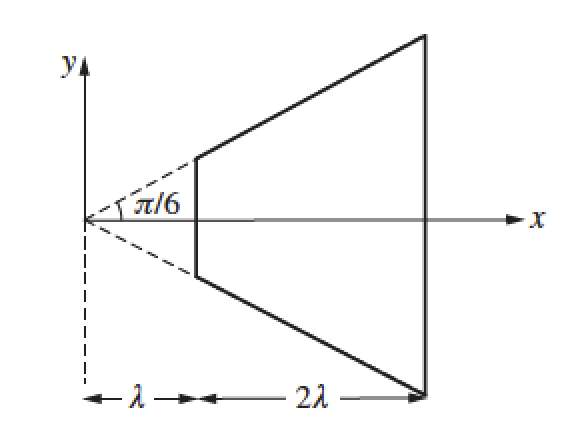
\includegraphics[width=6cm]{figures/BatinCavity.png}
	\centering
	\caption{Our electromagnetic bat is safe between these four walls.}
\end{figure}

\subsubsection{E: Rectangular Waveguide and its Modes}\label{E: Rectangular Waveguide and its Modes}

\textbf{\textcolor{red}{UNDER CONSTRUCTION}}
\subsubsection{E: Mirror mirror on the wall...}\label{E: Mirror mirror on the wall...}

\textbf{1):}

The boundary conditions that both fields have to satisfy on the surface of a perfect conductor are just:

\begin{equation}
	\mathbf{E}_{\parallel} =0, \quad \quad \quad \mathbf{B}_{\perp} = 0.
\end{equation}

\textbf{2):}

We know that we have to find a solution to:

\begin{equation}\label{waveeq}
	\left(\nabla^{2}_{\perp} +\gamma^{2}\right) \Psi = 0,
\end{equation}

that we have to solve for the each of the modes (a.k.a different boundary solutions). We already know that $\sin$ and $\cos$ are eigenfunctions for $\partial^{2}_{i}$ operator. This will help us to construct the form of the solution, as we will impose the field boundary conditions given by the conductor wall properties to determine if we need one trigonometric function or the other.
	
\subsubsection*{TM modes}

We have $E_{z}(x,y) =0$ at the boundaries. Also, we want the parallel component of $\mathbf{E} =0$ when $x=y=0$, so when we are in one of the corners. $\cos$ is not a 0 at this corner, so our solution to (\ref{waveeq}) looks like:

\begin{equation}
	E_{z} (x,y) = E_{0}\sin\left(\tfrac{\pi n x}{a}\right) \sin\left(\tfrac{\pi m y}{a}\right).
\end{equation}

This will give a cut-off of the form:

\begin{equation}\label{cutoff}
	\gamma^{2} = \tfrac{\pi^{2}}{a^{2}}\left(n^{2}+m^{2}\right).
\end{equation}

\subsubsection*{TE modes}

Same story here. Now, the boundary condition is that $\hat{n}\cdot \vec{\nabla}_{T}B^{z}(x,y) =0$ at the walls of the conductor. So we require the $\cos$ function as:

\begin{equation}
	B_{z}(x,y) = B_{0} \cos\left(\tfrac{\pi n x}{a}\right)\cos\left(\tfrac{\pi m y}{a}\right).
\end{equation}

With exactly the same cut-off frecuency $\gamma^{2}$ as before.

\textbf{3):}

Why do different modes have the same cut-off frequency? Just take a look at expression (\ref{cutoff}). If one interchanges $n,m$ values, the result is the same, but not the modes of $\mathbf{B}_{n,m}$ and $\mathbf{B}_{m,n}$. So basically, there is a symmetry in expression (\ref{cutoff}).

Actually, we can exploit this symmetry to craft modes that can be allowed in the second scenario, when one cuts the waveguide through the diagonal. In this case we want to impose that the fields, depending on the modes we study, are 0 in the line $x+y =a$.

\subsubsection*{TM modes}

Here we need to impose that $E_{z} =0$ on that line. Let's blindly follow the statement and generate a general linear combination with both possibilities.

\begin{equation}\label{LCfield}
	E_{z} = E^{(1)}_{0}\sin\left(\tfrac{\pi n x}{a}\right) \sin\left(\tfrac{\pi m y}{a}\right) + E^{2}_{0}\sin\left(\tfrac{\pi m x}{a}\right) \sin\left(\tfrac{\pi n y}{a}\right).
\end{equation}

We know that this expression should be equal to 0 when $y = a- x$.  If we evaluate there and use double angle trigonometric identities in wise way, we arrive to the following expression:

\begin{equation}
	\begin{split}
		0 = E_{z}|_{y= a- x} &= E^{(1)}_{0}\sin\left(\tfrac{\pi n x}{a}\right) (-1)^{m+1} \sin\left(\tfrac{\pi m x}{a}\right) + E^{2}_{0}\sin\left(\tfrac{\pi m x}{a}\right)(-1)^{n+1} \sin\left(\tfrac{\pi n x}{a}\right) \rightarrow\\
		E^{(2)} &= (-1)^{m+n+1} E^{(1)}_{0}.
	\end{split}
\end{equation}

So the expression in this case for a triangular waveguide is:

\begin{equation}
	E_{z} = E_{0}\left(\sin\left(\tfrac{\pi n x}{a}\right) \sin\left(\tfrac{\pi m y}{a}\right) + (-1)^{n+m+1}\sin\left(\tfrac{\pi m x}{a}\right) \sin\left(\tfrac{\pi n y}{a}\right)\right).
\end{equation}

\subsubsection*{TE modes}

Same story here. In this case the conditions will come from $(\partial_{x} + \partial_{y})B_{z} =0$. If we craft a general linear combination for the expression of the magnetic field as we did in (\ref{LCfield}), compute its derivates and plug those requirements into this linear combination expression, we will get:

\begin{equation}
	B_{z} = B_{0}\left(\cos\left(\tfrac{\pi n x}{a}\right) \cos\left(\tfrac{\pi m y}{a}\right) + (-1)^{n+m}\cos\left(\tfrac{\pi m x}{a}\right) \cos\left(\tfrac{\pi n y}{a}\right)\right).
\end{equation}

Powerful symmetry to exploit, is it not? 
	
	





